\documentclass[12pt, letterpaper]{article}
\usepackage[utf8]{inputenc}
\usepackage{graphicx}
\usepackage[margin=1in]{geometry}
\usepackage[font=small]{caption} 
\usepackage[font=footnotesize]{subcaption}
\title{Read Digits in Natural Scene Images using Convolutional Neural Networks }
\author{Ramesh Kumar(Matr. Nr. 9029726) \\ Roberto Cai Wu(Matri. Nr. 9029544 )}
\date{\today}
\begin{document}
\begin{titlepage}
\maketitle
\end{titlepage}

\section{Motivation}
\textbf{How this project related to Computed Vision?}
	\begin{itemize}
		\item Since computer vision is about interpreting the images from the camera such as image processing, classifying images based on features, etcetera.
		\item In this project, we also use computer vision methods for pre-processing and post-processing such as image size reduction, image conversion, and many more,  other than convolutional neural network. 
				\item Digit recognition is a computer vision problem used in applications such as postal mail sorting, bank check processing, form data entry, etcetera. 
	\end{itemize}



\textbf{Why Convolutional Neural Network}
	\begin{itemize}
		\item Since fast processing, accuracy and speed for these applications is important therefore, convolutional neural network is useful in this case.
		\item Furthermore, according to state-of-the-art, it shows better performance as compare to other approaches\cite{Convolutional Neural Networks Applied to House Numbers Digit Classification}
	\end{itemize}
 %therefore in our case,  pre-processing of images from the dataset can be done by using openCV library such as image size reduction, image cropping, etcetera, before feeding it to the convolutional neural network. We use convolutional network because  Furthermore, post-processing if needed can also be done by computer vision techniques. Lastly, for real time, camera feed and conversion of live images into gray scale 

%% Approach

\section{Approach}
The first part of this task consists of gathering data to train the network. We will use publicly available dataset; MNIST. Later on, we explain about this dataset in more details.  
Images from dataset will be preprocessed before feeding to the network. Later on, post-processing will be needed in cases where an image contains multiple digits to get a final result. 
\begin{itemize}
	\item Few possible approaches to solve this task are:
		\begin{itemize}
			\item Multiple hand-crafted features
			\item Template matching
			\item Convolutional Neural Network(we use this)
		\end{itemize}
	%\item Convolutional Neural Networks are used to extract features
	%from the images and classify them. These networks are %consists of different layers such as convolutional layers, pooling layers, and fully connected layers. Convolutional layer is first layer of the network that takes input as image and fully connected layer is final layer/output layer of the network that provides possible outcome based on input image.
	%\item  \textbf{Challenges}
	%	\begin{itemize}
	%		\item Different Lighting conditions
	%		\item Design an appropriate network
	%		\item Different perspective view
	%		\item Blurred digits 
	%		\item Can be more when we start implementation
			
	%	\end{itemize}
	%\item For testing, we will test the images from live camera under various possible conditions such as hand-written digits, computerized-written digits, different lighting conditions, different font sizes, etcetera.
	%\item Possible outcomes will be within 10 digit classes; one for each digit from label ``0'' to ``9'' and probability score of each outcome.
	%\item Furthermore outcome will also include locations of all recognized digits as well as information about what digits belong together and form a complete number
\end{itemize}

\subsection{Modified National Institute of Standards and Technology(MNIST) DataSet}

This dataset we use for our project to train the convolution network and predict in real time. It was created by National Institute of Standards and Technology(NIST). It consists of 60,000 training examples; each digit has 6,000 images, and testing examples of 10,000 examples. Furthermore, this dataset is size-normalized and centered to a fixed-size image. This dataset is mostly used by people who are interested to learn about pattern recognition methods or machine learning by devoting minimum amount of time on pre-processing and formatting the images. Each image in dataset contains one digit, and all digits are handwritten. Sample images of data set is shown in figure.


\subsection{Limitations}
	\begin{itemize}
		\item Images contain only digits.
		\item Background is a solid color and does not change. (Black or white)
		\item Number should be distanced enough so that bounding boxes do not overlap with other number.
	\end{itemize}

\begin{figure}[!h]
	\begin{center}	
		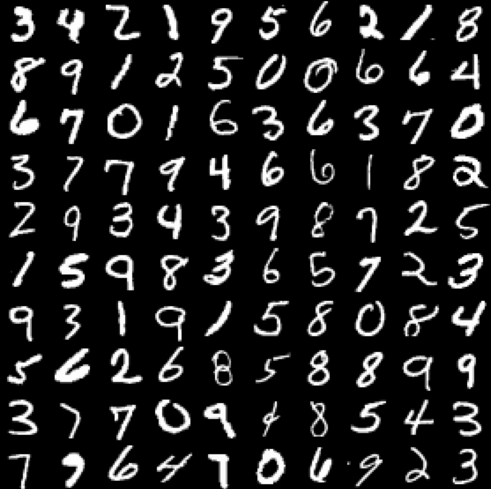
\includegraphics[scale = 0.5]{mnist-digits-small.png}
		\caption{ \cite{Classifying MNIST Digits} Samples images of MNIST dataset }
	\end{center}
\end{figure}  

\subsection{Graphic user interface (GUI)}
	We have designed a GUI to control the parameters for the binary threshold and the canny edge detector. The GUI can also show the images through different stages of the pre-processing steps. This is selected by a drop-down menu which contains the following options:
	\begin{itemize}
		\item Original: show the rgb image without any filter.
		\item Gray: show the image converted to gray-scale.
		\item Threshold: image after application of the binary threshold.
		\item Edge: shows the edge map.
		\item Median: shows threshold image after a median filter with 5x5 kernel.
		\item Contours: image with extracted contours.
		\item Bbox: shows original image with bounding boxes drawn around detected contours with the prediction.
	\end{itemize}
	
\begin{figure}[!h]
	\begin{center}	
	\begin{subfigure}{0.9\textwidth}
	\centering
	\includegraphics*[width=1 \textwidth]{tk_015.png}
	\end{subfigure}
		
	\end{center}
	\caption{ Graphic user interface.}
	\label{fig:gui}
\end{figure}  

\subsection{Pre-Processing}

\subsubsection{Pre-Processing of DataSet}

Since each image contain single digit with their label, therefore, we just do little pre-processing. First, we convert every image to the fixed size of (28,28,1) for faster computations. Then, we normalize all the images to make sure all pixels lies within one range. To make things easier for network, each image along with its label is converted from 1-dimensional class array to 10-dimensional class matrices by using Keras utility function.

\subsubsection{Pre-Processing of Live Images} 

For image pre-processing, we apply a series of filters to the image and detect contours that will represent the numbers. The first step is to resize the image to 1040x720 since we are using a cell phone camera to record and the original resolution exceeds the screen resolution. We pre-process first by converting the image into gray-scale and apply a Gaussian filter with a 5x5 kernel to smooth the image. The next step is to apply a binary threshold and since the background is constant (solid color), we can adjust the threshold to highlight the numbers. We then use the threshold image to compute an edge map via the Canny edge detector. 

\begin{figure}[!h]
\begin{center}
\begin{subfigure}{0.47\textwidth}
\centering
\includegraphics*[width=0.95 \textwidth, height=4cm]{thresh.png}
\caption{Binary threshold image}
\end{subfigure}
\begin{subfigure}{0.47\textwidth}
\centering
\includegraphics*[width=0.95 \textwidth, height=4cm]{edge.png}
\caption{Edge map with Canny edge detector}
\end{subfigure}
\end{center}
\caption{Images from first pre-processing steps.}
\label{fig:first-pre}
\end{figure}

The next step is to localize and extract the numbers from the image. For this we extract the contours from the edge map and only take the contours with an area bigger than 20 pixels. After obtaining the contours, we draw a bounding box surrounding each contour and crop each rectangle. Each rectangle is resized to a 28x28 and feed to the CNN classifier.
\begin{figure}[!h]
\begin{center}
\begin{subfigure}{0.47\textwidth}
\centering
\includegraphics*[width=0.95 \textwidth, height=4cm]{count.png}
\caption{Extracted contours.}
\end{subfigure}
\begin{subfigure}{0.47\textwidth}
\centering
\includegraphics*[width=0.95 \textwidth, height=4cm]{bbox.png}
\caption{Bounding box drawn over original image.}
\end{subfigure}
\end{center}
\caption{Images from second pre-processing steps.}
\label{fig:first-pre}
\end{figure}


\subsection{Keras Library}

In order to construct Convolutional Neural Network(CNN) model, we use Keras library. It is python deep learning library running on top of TensorFlow and Theano. We use Keras because it supports CNN and recurrent networks, and it is easier to use. It also runs on central processing unit(CPU) and graphics processing unit(GPU)\cite{keras}. 


\subsection{Convolutional Neural Network(CNN)}

Convolutional neural networks are made up of neurons that have adjustable weights and biases. Each neuron receives input, perform a dot product with weights and apply activation function to it; usually we use Rectified Linear Unit (ReLU). These networks assume that inputs are always images. Features are extracted to determine information about the image. Furthermore, layers in CNN are arranged in 3 dimensions: width, height, depth. These networks have ability to reduce the amount of parameters; such as weights and biases, without loosing any valuable information. This also helps for faster computations\cite{features_map}\cite{cnn_info}. 

\subsubsection{Architecture}

CNN architecture is mainly consists of three main layers arranged in sequential order:

\begin{itemize}
	\item Convolutional layer: This is first layer of network. It performs convolution operation with each pixel based on filter size. Filter contains random values initially(which can be considered as weights), each number in filter is multiplied with its corresponding pixel in image. After that, all values inside filter are added, we get only single number. Figure \ref{features} gives clear idea how this works. Here size of our filter is 5 by 5, after multiplication and addition, we get one number which we can see in right side of image. This process is performed on every location of image. So, we get important features of image, and these important features are fed to next layer for further processing. Furthermore, we can also use more than one convolution layer, it depends upon complexity of image. Lastly, weights inside filters are adjusted according to back-propagation algorithm; where first we computed error between current output and desired output, and based on error we adjust our weights to get more closer to our desired output.
	
	\begin{figure}[!h]
		\begin{center}	
			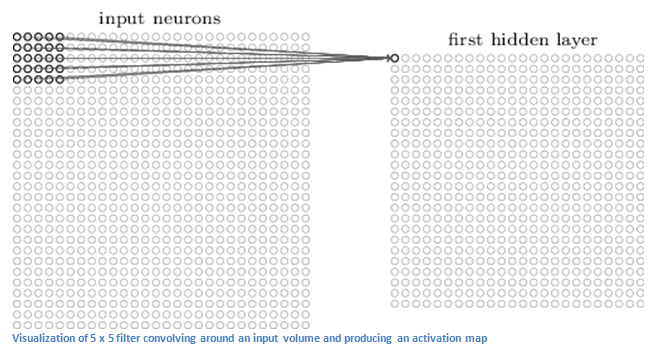
\includegraphics[scale = 0.8]{ActivationMap.png}
			\caption{ \cite{features_map} Visualization of 5 by 5 filter } \label{features}
		\end{center}
	\end{figure}  
		
	\item Pooling layer: The main purpose of this layer is to reduce the size of image. This helps in reducing amount of parameters, which requires less computation and also reduction in variance in image. Furthermore, pooling is achieved into two different ways; max and average pooling. Max pooling considers element with maximum value inside filter. While, average pooling computes average of all elements inside filter and replace average value in image.
	\item Fully-Connected layer: This layer takes input from previous layer; can be convolution or pooling layer and convert output of network according to number of classes. In our case, we have 10 classes; 0 to 9. so it outputs 10 values along with the probability of each digit. This is done by using soft-max activation function, which returns probabilities. \cite{features_map}\cite{cnn_info}
\end{itemize}

Figure \ref{model} below shows block diagram that we used to train the 
model. 

\begin{figure}[!h]
	\centering
	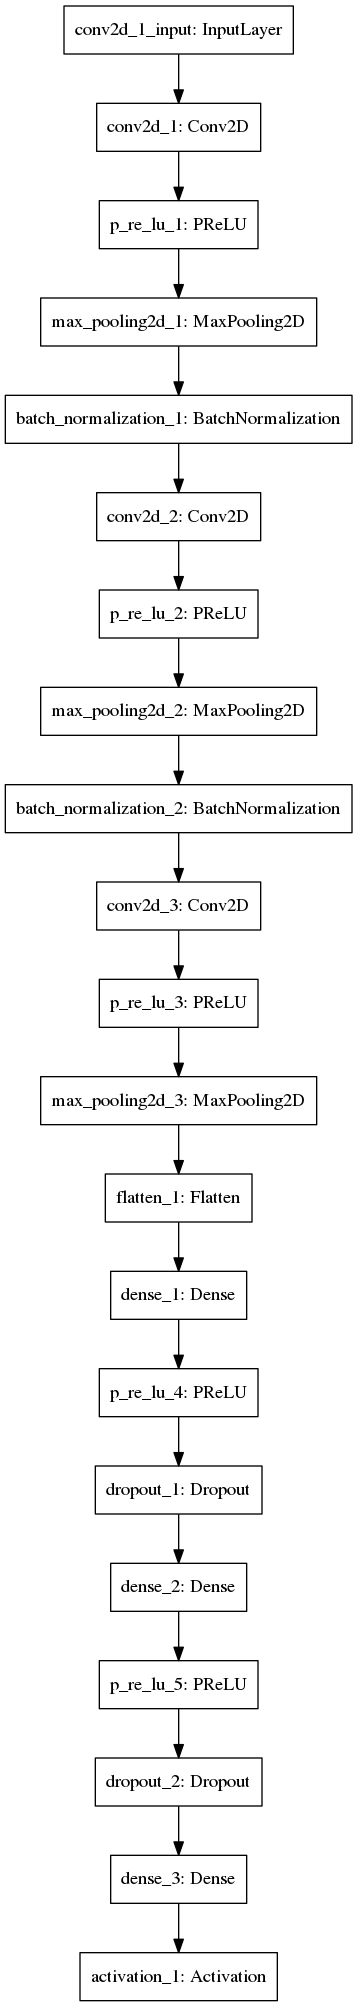
\includegraphics[scale = 0.25]{trained_model_diagram.png}
	
	\caption{CNN Model used to train MNIST dataset} \label{model}
\end{figure}
\newpage
\subsection{Post-Processing}

The post-processing consists of handling the predicted number for each cropped image sent to the CNN classifier. Once we have the predicted number, we draw the predicted number over the corresponding bounding box. An example image is shown in Figure \ref{fig:pred}.

\begin{figure}[!h]
\begin{center}
\begin{subfigure}{0.47\textwidth}
\centering
\includegraphics*[width=0.95 \textwidth, height=4cm]{bbox_p2.png}
\end{subfigure}
\end{center}
\caption{Image with number prediction.}
\label{fig:pred}
\end{figure}


\subsection{Challenges}

	\begin{itemize}
		\item Different Lighting conditions
		\item Shadows
		\item Distance between multi-digits(If digits are too close, then contour detection becomes incorrect, which also affects classification by CNN)
		\item Different perspective view
		\item Occluded and blurred digits
	\end{itemize}

\subsection{Results}

After training on 60,000 samples images and testing on 10,000 images, we got accuracy of 99.13\%. \\
Furthermore, we also tested on real time, and classification results are satisfy.
(attach figure of classification using real time here)

%\section{Contribution}

%\begin{itemize}
%	\item Pre-processing using available dataset(Roberto Cai)
%	\item Create the dataset and integrate with publicly available dataset (Ramesh Kumar)
%	\item Create the Network(pair)
%	\item Post-processing (Roberto Cai)
%	\item Probability Score (Ramesh Kumar)
%	\item Individual number combination in final result (Roberto Cai)
%	\item Evaluation of approach (Ramesh Kumar)
%	\item Documentation(pair)
%\end{itemize}
\newpage
\begin{thebibliography}{9}
\bibitem{Convolutional Neural Networks Applied to House Numbers Digit Classification}
Pierre Sermanet, Soumith Chintala and Yann LeCun, "Convolutional Neural Networks Applied to
House Numbers Digit Classification", The Courant Institute of Mathematical Sciences - New York University 

\bibitem{Reading Digits in Natural Images
	with Unsupervised Feature Learning}

Yuval Netzer
, Tao Wang
, Adam Coates
, Alessandro Bissacco1
, Bo Wu
, Andrew Y. Ng, "Reading Digits in Natural Images
with Unsupervised Feature Learning", In NIPS Workshop on Deep
Learning and Unsupervised Feature Learning, 2011.

\bibitem{Classifying MNIST Digits}

http://theanets.readthedocs.io/en/stable/examples/mnist-classifier.html

\bibitem{keras}
https://keras.io/

\bibitem{features_map}
https://adeshpande3.github.io/adeshpande3.github.io/A-Beginner\%27s-Guide-To-Understanding-Convolutional-Neural-Networks/
\bibitem{cnn_info}
http://cs231n.github.io/convolutional-networks/

\end{thebibliography} 

\end{document}